%pdflatex abra.tex
%convert -density 150x150 abra.pdf abra.png
\documentclass[border={2pt 2pt 2pt 2pt}]{standalone}
\usepackage{tikz}
\usetikzlibrary{calc}
\begin{document}

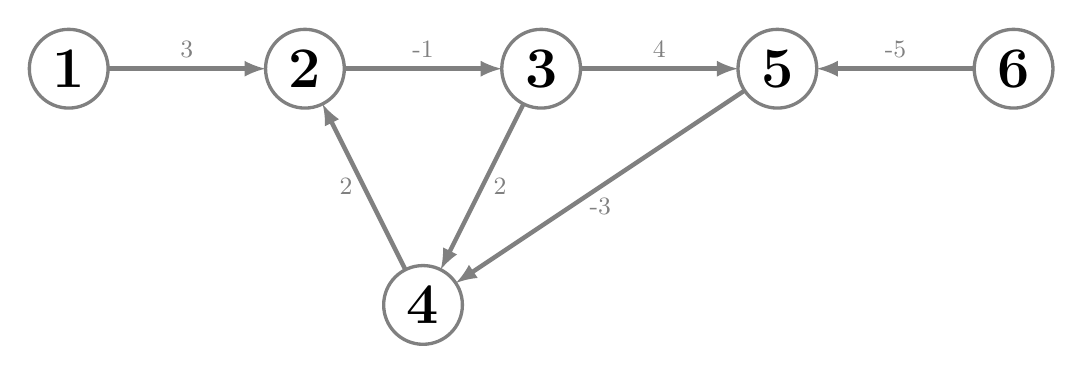
\begin{tikzpicture}
\coordinate (A) at (0,3);
\coordinate (B) at (3,3);
\coordinate (C) at (6,3);
\coordinate (D) at (4.5,0);
\coordinate (E) at (9,3);
\coordinate (F) at (12,3);
\draw[gray,ultra thick,-latex,shorten >=0.5cm] (A)--(B) node [gray,midway, above] {\small 3};
\draw[gray,ultra thick,-latex,shorten >=0.5cm] (B)--(C) node [gray,midway, above] {\small -1};
\draw[gray,ultra thick,-latex,shorten >=0.5cm] (C)--(D) node [gray,midway,right] {\small 2};
\draw[gray,ultra thick,-latex,shorten >=0.5cm] (D)--(B) node [gray,midway,left] {\small 2};
\draw[gray,ultra thick,-latex,shorten >=0.5cm] (C)--(E) node [gray,midway, above] {\small 4};
\draw[gray,ultra thick,-latex,shorten >=0.5cm] (E)--(D) node [gray,midway, below] {\small -3};
\draw[gray,ultra thick,-latex,shorten >=0.5cm] (F)--(E) node [gray,midway, above] {\small -5};
\draw[gray,very thick,fill=white] (A) circle [radius=0.5];
\draw[gray,very thick,fill=white] (B) circle [radius=0.5];
\draw[gray,very thick,fill=white] (C) circle [radius=0.5];
\draw[gray,very thick,fill=white] (D) circle [radius=0.5];
\draw[gray,very thick,fill=white] (E) circle [radius=0.5];
\draw[gray,very thick,fill=white] (F) circle [radius=0.5];
\node at (A) {\huge\bf 1};
\node at (B) {\huge\bf 2};
\node at (C) {\huge\bf 3};
\node at (D) {\huge\bf 4};
\node at (E) {\huge\bf 5};
\node at (F) {\huge\bf 6};
\end{tikzpicture}
\end{document}
